\documentclass{beamer}
% =============================================================================
% ENCODING
% =============================================================================
\usepackage[utf8]{inputenc}  % UTF-8 encoding support

% =============================================================================
% GRAPHICS
% =============================================================================
\usepackage{graphicx}  % For \includegraphics (401 uses across lectures)

% =============================================================================
% MATH PACKAGES
% =============================================================================
\usepackage{amsmath}    % For align, multline, equation environments (heavily used)
\usepackage{amsfonts}   % For \mathbb (e.g., \bbR, \bbE)
\usepackage{amssymb}    % For additional math symbols

% =============================================================================
% TABLES
% =============================================================================
\usepackage{booktabs}   % For \toprule, \midrule, \bottomrule (used in lecture13, lecture14)

% =============================================================================
% LISTS
% =============================================================================
\usepackage{enumerate}  % Enhanced enumerate environment (76 uses across lectures)

% =============================================================================
% TIKZ (DIAGRAMS)
% =============================================================================
\usepackage{tikz}       % For taxonomy diagram and footnotes positioning

% =============================================================================
% UTILITY PACKAGES
% =============================================================================
\usepackage{multido}    % For \multido command used in \eqpause
\usepackage{etoolbox}   % For \AtEndEnvironment, \ifbool, \newbool (used in preamble and taxonomy)

% =============================================================================
% BEAMER THEME SETTINGS
% =============================================================================
\usetheme{default}
\usecolortheme{default}

\setbeamerfont{title}{size=\Huge}
\setbeamertemplate{footline}[frame number]{}
\setbeamertemplate{section in toc}[sections numbered]

\makeatletter
\newcommand\HUGE{\@setfontsize\Huge{35}{40}}
\makeatother    

\setbeamerfont{title}{size=\HUGE}
\beamertemplatenavigationsymbolsempty

% =============================================================================
% TIKZ LIBRARIES
% =============================================================================
% Used for taxonomy diagram: arrows, positioning, shapes
\usetikzlibrary{arrows.meta,calc,shapes,positioning,shadows,trees}

% =============================================================================
% CUSTOM FOOTNOTE COMMANDS
% =============================================================================
% \myfootnote{text} - creates a footnote at the bottom of the slide
\newcommand\myfootnote[1]{%
  \vspace{-0.5cm}%
  \tikz[remember picture,overlay]
  \draw (current page.south west) +(1in + \oddsidemargin,0.5em)
  node[anchor=south west,inner sep=0pt]{\parbox{\textwidth}{%
      \rlap{\rule{10em}{0.4pt}}\raggedright\scriptsize \textit{#1}}};}

% \myfootnotewithlink{url}{text} - creates a clickable footnote (623 uses across lectures)
\newcommand\myfootnotewithlink[2]{%
  \vspace{-0.5cm}%
  \tikz[remember picture,overlay]
  \draw (current page.south west) +(1in + \oddsidemargin,0.5em)
  node[anchor=south west,inner sep=0pt]{\parbox{\textwidth}{%
      \rlap{\rule{10em}{0.4pt}}\raggedright\scriptsize\href{#1}{\textit{#2}}}};}

% =============================================================================
% SECTION/SUBSECTION OUTLINE AUTOMATION
% =============================================================================
% Automatically show outline at the beginning of each section
\AtBeginSection[]
      {
      	\begin{frame}{Outline}
      		\tableofcontents[currentsection]
      	\end{frame}
      }
      \AtBeginSubsection[]{
      	\begin{frame}{Outline}
      		\tableofcontents[currentsection,currentsubsection]
      	\end{frame}
}

% =============================================================================
% CUSTOM SLIDE ANIMATION COMMANDS
% =============================================================================
% These commands enable step-by-step reveal of equations and content
% Used heavily across all lectures (1130+ uses of \nextonslide and \eqpause)

\newcounter{noscounter}   % Counter for \nextonslide (resets on each new slide)
\newcounter{pcounter}     % Counter for pause commands (resets after \eqpause)
\newcounter{diffcounter}  % Counts pauses after equations

% \nextonslide{content} - reveals content on the next overlay
\newcommand{\nextonslide}[1]{%
  \stepcounter{noscounter}%
  \stepcounter{pcounter}%
  \stepcounter{diffcounter}%
  \onslide<\value{noscounter}->{#1}%
}

% \resetonslide - resets all animation counters (called at each frame)
\newcommand{\resetonslide}{%
    \setcounter{noscounter}{1}%
    \setcounter{pcounter}{1}%
    \setcounter{diffcounter}{0}%
}

% \eqpause - pause after equation that syncs with \nextonslide
\newcommand{\eqpause}{%
  \multido{\i=1+1}{\value{pcounter}}{\pause}%
  \stepcounter{noscounter}%
  \setcounter{pcounter}{1}%
}

% \eqpausediff - helper command, runs automatically after math environments
\newcommand{\eqpausediff}{%
  \multido{\i=1+1}{\value{diffcounter}}{\pause}%
  \addtocounter{pcounter}{-\value{diffcounter}}%
  \setcounter{diffcounter}{0}%
}

% Apply \eqpausediff after math environments
\newcommand\AtEndBoth[2]{%
  \AtEndEnvironment{#1}{#2}%
  \AtEndEnvironment{#1*}{#2}%
}

\AtEndBoth{align}{\eqpausediff}
\AtEndBoth{equation}{\eqpausediff}
\AtEndBoth{multline}{\eqpausediff}

% Reset counters at the beginning of each frame
\addtobeamertemplate{frametitle}{\resetonslide}{}

% =============================================================================
% INCLUDE OTHER CONFIGURATION FILES
% =============================================================================
% ==============================================================================
% Custom LaTeX Commands for Deep Generative Models Course
% ==============================================================================

% ==============================================================================
% BOLD LETTERS (mathbf / boldsymbol)
% ==============================================================================

% ------------------------------------------------------------------------------
% Latin Bold Lowercase
% Usage: \bx for x in bold, commonly used for vectors
% ------------------------------------------------------------------------------
\newcommand{\ba}{\mathbf{a}}
\newcommand{\bc}{\mathbf{c}}
\newcommand{\be}{\mathbf{e}}
\newcommand{\bff}{\mathbf{f}}  % Note: \bf is reserved for bold font switching
\newcommand{\bg}{\mathbf{g}}
\newcommand{\bh}{\mathbf{h}}
\newcommand{\bp}{\mathbf{p}}
\newcommand{\bq}{\mathbf{q}}
\newcommand{\bs}{\mathbf{s}}
\newcommand{\bt}{\mathbf{t}}
\newcommand{\bu}{\mathbf{u}}
\newcommand{\bv}{\mathbf{v}}
\newcommand{\bw}{\mathbf{w}}
\newcommand{\bx}{\mathbf{x}}
\newcommand{\by}{\mathbf{y}}
\newcommand{\bz}{\mathbf{z}}

% ------------------------------------------------------------------------------
% Latin Bold Uppercase
% Usage: \bX for X in bold, commonly used for matrices or random vectors
% ------------------------------------------------------------------------------
\newcommand{\bA}{\mathbf{A}}
\newcommand{\bG}{\mathbf{G}}
\newcommand{\bI}{\mathbf{I}}
\newcommand{\bJ}{\mathbf{J}}
\newcommand{\bL}{\mathbf{L}}
\newcommand{\bM}{\mathbf{M}}
\newcommand{\bP}{\mathbf{P}}
\newcommand{\bQ}{\mathbf{Q}}
\newcommand{\bR}{\mathbf{R}}
\newcommand{\bT}{\mathbf{T}}
\newcommand{\bU}{\mathbf{U}}
\newcommand{\bV}{\mathbf{V}}
\newcommand{\bW}{\mathbf{W}}
\newcommand{\bX}{\mathbf{X}}
\newcommand{\bZ}{\mathbf{Z}}

% ------------------------------------------------------------------------------
% Greek Bold Lowercase
% Usage: \btheta for θ in bold, commonly used for parameter vectors
% ------------------------------------------------------------------------------
\newcommand{\bepsilon}{\boldsymbol{\epsilon}}
\newcommand{\blambda}{\boldsymbol{\lambda}}
\newcommand{\bmu}{\boldsymbol{\mu}}
\newcommand{\bphi}{\boldsymbol{\phi}}
\newcommand{\bpi}{\boldsymbol{\pi}}
\newcommand{\bpsi}{\boldsymbol{\psi}}
\newcommand{\bsigma}{\boldsymbol{\sigma}}
\newcommand{\btheta}{\boldsymbol{\theta}}

% ------------------------------------------------------------------------------
% Greek Bold Uppercase
% Usage: \bSigma for Σ in bold, commonly used for covariance matrices
% ------------------------------------------------------------------------------
\newcommand{\bSigma}{\boldsymbol{\Sigma}}
\newcommand{\bTheta}{\boldsymbol{\Theta}}

% ==============================================================================
% CALLIGRAPHIC LETTERS (mathcal)
% Usage: \cX for calligraphic X, commonly used for sets and spaces
% ==============================================================================
\newcommand{\cF}{\mathcal{F}}
\newcommand{\cI}{\mathcal{I}}
\newcommand{\cL}{\mathcal{L}}
\newcommand{\cM}{\mathcal{M}}
\newcommand{\cN}{\mathcal{N}}
\newcommand{\cP}{\mathcal{P}}
\newcommand{\cS}{\mathcal{S}}
\newcommand{\cT}{\mathcal{T}}
\newcommand{\cW}{\mathcal{W}}
\newcommand{\cX}{\mathcal{X}}
\newcommand{\cZ}{\mathcal{Z}}

% ==============================================================================
% BLACKBOARD BOLD LETTERS (mathbb)
% Usage: \bbR for ℝ, commonly used for number sets and expectations
% ==============================================================================
\newcommand{\bbE}{\mathbb{E}}  % Expectation
\newcommand{\bbI}{\mathbb{I}}  % Indicator function
\newcommand{\bbP}{\mathbb{P}}  % Probability measure
\newcommand{\bbR}{\mathbb{R}}  % Real numbers

% ==============================================================================
% MATH OPERATORS
% ==============================================================================

% ------------------------------------------------------------------------------
% Optimization Operators
% Usage: \argmin_{x} f(x) for proper spacing and limits placement
% ------------------------------------------------------------------------------
\DeclareMathOperator*{\argmin}{arg\,min}
\DeclareMathOperator*{\argmax}{arg\,max}

% ------------------------------------------------------------------------------
% Statistical Operators
% Usage: \cov(X, Y) for covariance
% ------------------------------------------------------------------------------
\DeclareMathOperator{\cov}{cov}

% ------------------------------------------------------------------------------
% Linear Algebra Operators
% Usage: \tr(\bA) for trace of matrix A
% ------------------------------------------------------------------------------
\DeclareMathOperator{\tr}{tr}

% ------------------------------------------------------------------------------
% Other Mathematical Operators
% ------------------------------------------------------------------------------
\DeclareMathOperator{\diver}{div}      % Divergence (vector calculus)
\DeclareMathOperator{\softmax}{softmax}
\DeclareMathOperator{\supp}{supp}      % Support of a distribution

% ==============================================================================
% PROBABILITY DISTRIBUTIONS
% Usage: X \sim \cN(0, 1), Y \sim \Bern(p)
% ==============================================================================
\DeclareMathOperator{\Bern}{Bern}      % Bernoulli distribution
\DeclareMathOperator{\Cat}{Cat}        % Categorical distribution
\DeclareMathOperator{\Gumbel}{Gumbel}  % Gumbel distribution
\DeclareMathOperator{\Uniform}{Uniform}

% ==============================================================================
% METRICS AND DIVERGENCES
% Usage: \KL(p \| q), \JSD(p, q)
% ==============================================================================
\newcommand{\Ent}{\mathrm{H}}          % Entropy
\newcommand{\FID}{\mathrm{FID}}        % Fréchet Inception Distance
\newcommand{\JSD}{\mathrm{JSD}}        % Jensen-Shannon Divergence
\newcommand{\KL}{\mathrm{KL}}          % Kullback-Leibler Divergence
\DeclareMathOperator{\MMD}{MMD}        % Maximum Mean Discrepancy
\DeclareMathOperator{\SNR}{SNR}        % Signal-to-Noise Ratio

% ==============================================================================
% NEURAL NETWORK NOTATION
% ==============================================================================

% ------------------------------------------------------------------------------
% Network Architectures (upright font for abbreviations)
% Usage: f_{\btheta} = \NN_{\btheta}(\bx)
% ------------------------------------------------------------------------------
\newcommand{\MLP}{\mathrm{MLP}}        % Multi-Layer Perceptron
\newcommand{\NN}{\mathrm{NN}}          % Neural Network
\newcommand{\RNN}{\mathrm{RNN}}        % Recurrent Neural Network

% ------------------------------------------------------------------------------
% Numerical Solvers (monospace font)
% Usage: \bx_T = \ODESolve(f, \bx_0, T)
% ------------------------------------------------------------------------------
\newcommand{\ODESolve}{\texttt{ODESolve}}
\newcommand{\SDESolve}{\texttt{SDESolve}}

% ==============================================================================
% COMMON SHORTCUTS
% Usage: Frequently used subscripted or parameterized expressions
% ==============================================================================
\newcommand{\pd}{p_{\text{data}}}              % Data distribution
\newcommand{\pt}{p_{\boldsymbol{\theta}}}      % Parameterized distribution
\newcommand{\qagg}{q_{\text{agg}}}             % Aggregated posterior
\newcommand{\lambdamax}{\lambda_{\text{max}}}  % Maximum eigenvalue
  % Math shorthand commands (\bx, \bbE, \KL, etc.)
\input{../utils/title}        % Title page template
\centering
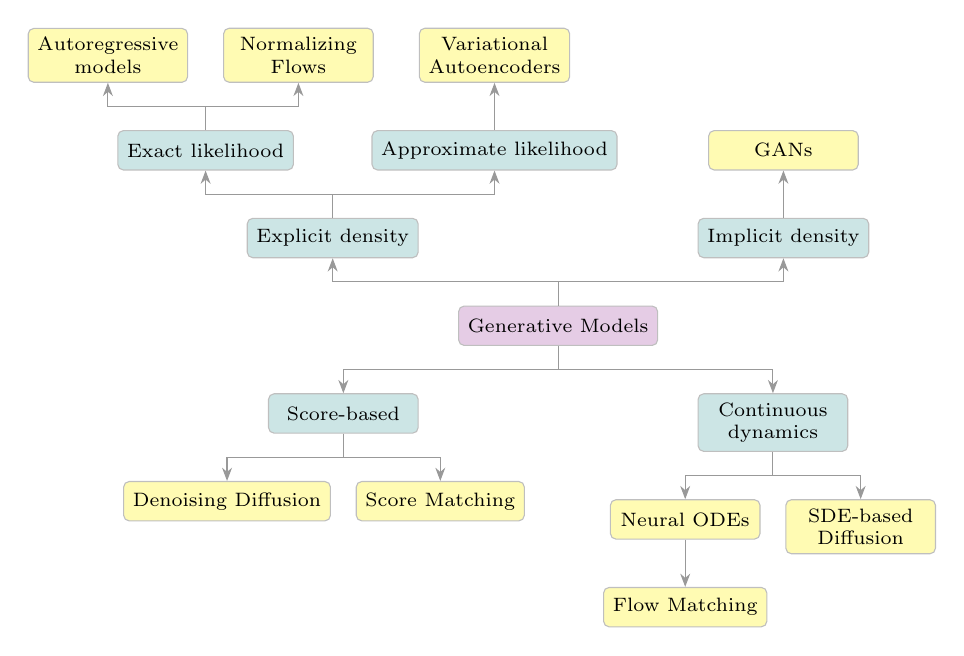
\begin{tikzpicture}[
    scale=1.0, transform shape,
    node distance=0.6cm and 0.3cm,
    box/.style={
        rectangle, 
        draw=gray!50, 
        rounded corners=2pt, 
        minimum width=1.9cm, 
        minimum height=0.5cm, 
        align=center, 
        font=\scriptsize, 
        line width=0.4pt
    },
    root/.style={box, fill=violet!20},
    category/.style={box, fill=teal!20},
    model/.style={box, fill=yellow!30},
    arrow/.style={-Stealth, draw=gray!80, line width=0.4pt}
]

    % --- CENTRAL ROOT ---
    \node[root] (root) {Generative Models};

    % --- UPPER BRANCHES (SWAPPED) ---
    % Tier 1: Explicit (Left) and Implicit (Right)
    \node[category, above left=0.6cm and 0.5cm of root] (explicit) {Explicit density};
    \node[category, above right=0.6cm and 0.5cm of root] (implicit) {Implicit density};

    % Tier 2 (Left side: Likelihoods)
    \node[category, above left=0.6cm and -0.6cm of explicit] (exact) {Exact likelihood};
    \node[category, above right=0.6cm and -0.6cm of explicit] (approx) {Approximate likelihood};

    % Tier 2 (Right side: GANs)
    \node[model, above=0.6cm of implicit] (gans) {GANs};

    % Tier 3 (Final Models Up)
    \node[model, above left=0.6cm and -0.9cm of exact] (ar) {Autoregressive \\ models};
    \node[model, above right=0.6cm and -0.9cm of exact] (nf) {Normalizing \\ Flows};
    \node[model, above=0.6cm of approx] (vae) {Variational \\ Autoencoders};

    % --- LOWER BRANCHES ---
    % Tier 1: Score-based and Continuous
    \node[category, below left=0.6cm and 0.5cm of root] (score) {Score-based};
    \node[category, below right=0.6cm and 0.5cm of root] (cont) {Continuous \\ dynamics};

    % Tier 2 (Score Models)
    \node[model, below left=0.6cm and -0.8cm of score] (ddpm) {Denoising Diffusion};
    \node[model, below right=0.6cm and -0.8cm of score] (sm) {Score Matching};

    % Tier 2 (Continuous Models)
    \node[model, below left=0.6cm and -0.8cm of cont] (node) {Neural ODEs};
    \node[model, below right=0.6cm and -0.8cm of cont] (sde) {SDE-based \\ Diffusion};

    % Tier 3 (Flow Matching)
    \node[model, below=0.6cm of node] (fm) {Flow Matching};

    % --- CONNECTIONS ---
    % Root to Tier 1
    \draw[arrow] (root.north) -- ++(0,0.3) -| (explicit.south);
    \draw[arrow] (root.north) -- ++(0,0.3) -| (implicit.south);
    \draw[arrow] (root.south) -- ++(0,-0.3) -| (score.north);
    \draw[arrow] (root.south) -- ++(0,-0.3) -| (cont.north);

    % Explicit side connections
    \draw[arrow] (explicit.north) -- ++(0,0.3) -| (exact.south);
    \draw[arrow] (explicit.north) -- ++(0,0.3) -| (approx.south);
    \draw[arrow] (exact.north) -- ++(0,0.3) -| (ar.south);
    \draw[arrow] (exact.north) -- ++(0,0.3) -| (nf.south);
    \draw[arrow] (approx.north) -- (vae.south);

    % Implicit side connection
    \draw[arrow] (implicit.north) -- (gans.south);

    % Score side connections
    \draw[arrow] (score.south) -- ++(0,-0.3) -| (ddpm.north);
    \draw[arrow] (score.south) -- ++(0,-0.3) -| (sm.north);

    % Continuous side connections
    \draw[arrow] (cont.south) -- ++(0,-0.3) -| (node.north);
    \draw[arrow] (cont.south) -- ++(0,-0.3) -| (sde.north);
    \draw[arrow] (node.south) -- (fm.north);

\end{tikzpicture}     % Generative models taxonomy diagram

\createdgmtitle{12}

%--------------------------------------------------------------------------------
\begin{document}
%--------------------------------------------------------------------------------
\begin{frame}[noframenumbering,plain]
\titlepage
	\resetonslide
\end{frame}
%=======
\begin{frame}{Recap of Previous Lecture}
	\myfootnotewithlink{https://arxiv.org/abs/2011.13456}{Song Y., et al. Score-Based Generative Modeling through Stochastic Differential Equations, 2020}
	\vspace{-0.3cm}
	\[
		d\bx = \bff(\bx, t) dt + g(t) d \bw
	\]
	\vspace{-0.3cm}
	\begin{block}{Variance Exploding SDE (NCSN)}
		\vspace{-0.5cm}
		\[
			d \bx = \sqrt{\frac{ d [\sigma^2(t)]}{dt}} \cdot d \bw, \quad \bff(\bx, t) = 0, \quad g(t) = \sqrt{\frac{ d [\sigma^2(t)]}{dt}} 
		\]
		The variance grows since $\sigma(t)$ is a monotonically increasing function.
	\end{block}
	\begin{block}{Variance Preserving SDE (DDPM)}
		\vspace{-0.3cm}
		\[
			d \bx = - \frac{1}{2} \beta(t) \bx(t) dt + \sqrt{\beta(t)} \cdot d \bw
		\]
		\[
			\bff(\bx, t) = - \frac{1}{2} \beta(t) \bx(t) , \quad g(t) = \sqrt{\beta(t)} 
		\]
		The variance is preserved if $\bx(0)$ has unit variance.
	\end{block}
\end{frame}
%=======
\begin{frame}{Recap of Previous Lecture}
	\myfootnotewithlink{https://arxiv.org/abs/2011.13456}{Song Y., et al. Score-Based Generative Modeling through Stochastic Differential Equations, 2020}
	\begin{block}{Discrete-Time Objective}
		\vspace{-0.3cm}
		\[
			\bbE_{\pd(\bx_0)} \bbE_{t \sim U\{1, T\}} \bbE_{q(\bx_t | \bx_0)}\bigl\| \bs_{\btheta, t}(\bx_t) - \nabla_{\bx_t} \log q(\bx_t | \bx_0) \bigr\|^2_2 
		\]
		\vspace{-0.5cm}
	\end{block}
	\begin{block}{Continuous-Time Objective}
		\vspace{-0.5cm}
		\[
			\bbE_{\pd(\bx(0))} \bbE_{t \sim U[0, 1]} \bbE_{q(\bx(t) | \bx(0))}\bigl\| \bs_{\btheta}(\bx(t), t) - {\color{teal}\nabla_{\bx(t)} \log q(\bx(t) | \bx(0))} \bigr\|^2_2 
		\]
		\vspace{-0.5cm}
	\end{block}
	\begin{block}{NCSN}
		\vspace{-0.3cm}
		\[
			q(\bx(t) | \bx(0)) = \cN\left(\bx(0), \left[\sigma^2(t) - \sigma^2(0)\right] \cdot \bI\right)
		\]
		\vspace{-0.5cm}
	\end{block}
	\begin{block}{DDPM}
		\vspace{-0.5cm}
		\[
			q(\bx(t) | \bx(0)) = \cN\left(\bx(0) e^{-\frac{1}{2} \int_0^t\beta(s)ds}, \left(1 - e^{- \int_0^t\beta(s)ds}\right) \cdot \bI\right)
		\]
	\end{block}
	
\end{frame}
%=======
\begin{frame}{Recap of Previous Lecture}
	\myfootnotewithlink{https://arxiv.org/abs/2011.13456}{Song Y., et al. Score-Based Generative Modeling through Stochastic Differential Equations, 2020}
	\begin{block}{Sampling}
		To sample, solve the reverse SDE using numerical solvers (\texttt{SDESolve}).
		\vspace{-0.3cm}
		\begin{figure}
			\includegraphics[width=0.8\linewidth]{figs/sbgm}
		\end{figure}
		\vspace{-0.5cm}
	\end{block}
	\begin{itemize}
		\item Discretizing the reverse SDE gives us ancestral sampling.
		\item If we use the probability flow ODE instead, then the reverse ODE yields DDIM sampling.
	\end{itemize}
\end{frame}
%=======
\begin{frame}{Recap of Previous Lecture}
	\myfootnotewithlink{https://arxiv.org/abs/2210.02747}{Lipman Y., et al. Flow Matching for Generative Modeling, 2022}
	Consider ODE dynamics $\bx(t)$ in the interval $t \in [0, 1]$ with $\bx_0 \sim p_0(\bx) = p(\bx)$, $\bx_1 \sim p_1(\bx) =  \pd(\bx)$.
	\[
		\frac{d \bx}{dt} = \bff (\bx, t),  \quad \text{with initial condition $\bx(0) = \bx_0$}.
	\]
	\vspace{-0.5cm}
	\begin{block}{KFP Theorem (Continuity Equation)}
		\vspace{-0.5cm}
		\[
			\frac{\partial p_t(\bx)}{\partial t} = - \text{div}\left(\bff(\bx, t) p_t(\bx)\right) \Leftrightarrow \frac{d \log p_t(\bx(t))}{d t} = - \text{tr} \left( \frac{\partial \bff(\bx(t), t)}{\partial \bx(t)} \right)
		\]
		\vspace{-0.5cm}
	\end{block}
	Solving the continuity equation using the adjoint method is complicated and unstable.
	\begin{block}{Flow Matching}
		\vspace{-0.3cm}
		\[
			\bbE_{t \sim U[0, 1]} \bbE_{\bx \sim p_t(\bx)}\left\| \bff(\bx, t) - \bff_{\btheta}(\bx, t) \right\|^2 \rightarrow \min_{\btheta}
		\]
		\vspace{-0.3cm}
	\end{block}
\end{frame}
%=======
\begin{frame}{Recap of Previous Lecture}
	\myfootnotewithlink{https://arxiv.org/abs/2302.00482}{Tong A., et al. Improving and Generalizing Flow-Based Generative Models with Minibatch Optimal Transport, 2023}
	\vspace{-0.3cm}
	Introduce the latent variable $\bz$:
	\[
		p_t(\bx) = \int p_t(\bx | \bz) p(\bz) d \bz 
	\]
	\vspace{-0.5cm}
	\[
		\frac{\partial p_t(\bx | \bz)}{\partial t} = - \text{div}\left(\bff(\bx, \bz, t) p_t(\bx | \bz)\right).
	\]
	\vspace{-0.3cm}
	\begin{itemize}
		\item $p_t(\bx | \bz)$ is a \textbf{conditional probability path}
		\item $\bff(\bx, \bz, t)$ is a \textbf{conditional vector field}
	\end{itemize}
	\[
		\frac{d\bx}{dt} = \bff(\bx, t) \quad \Rightarrow \quad \frac{d\bx}{dt} = \bff(\bx, \bz, t)
	\]
	\vspace{-0.5cm}
	\begin{block}{Theorem}
		The following vector field generates the probability path $p_t(\bx)$:
		\vspace{-0.2cm}
		\[
			\bff(\bx, t) = \bbE_{p_t(\bz | \bx)} \bff(\bx, \bz, t)  = {\color{teal}\int \bff(\bx, \bz, t)} \frac{\color{teal}p_t(\bx | \bz) p(\bz)}{p_t(\bx)} {\color{teal}d \bz}
		\]
		\vspace{-0.5cm}
	\end{block}
\end{frame}
%=======
\begin{frame}{Recap of Previous Lecture}
	\myfootnotewithlink{https://arxiv.org/abs/2302.00482}{Tong A., et al. Improving and Generalizing Flow-Based Generative Models with Minibatch Optimal Transport, 2023}
	\begin{block}{Flow Matching (FM)}
		\vspace{-0.5cm}
		\[
			\bbE_{t \sim U[0, 1]} \bbE_{\bx \sim p_t(\bx)}\left\| \bff(\bx, t) - \bff_{\btheta}(\bx, t) \right\|^2 \rightarrow \min_{\btheta}
		\]
		\vspace{-0.5cm}
	\end{block}
	\begin{block}{Conditional Flow Matching (CFM)}
		\vspace{-0.5cm}
		\[
			\bbE_{t \sim U[0, 1]} \bbE_{\bz \sim p(\bz)} \bbE_{\bx \sim p_t(\bx | \bz)}\left\| \bff(\bx, \bz, t) - \bff_{\btheta}(\bx, t) \right\|^2 \rightarrow \min_{\btheta}
		\]
		\vspace{-0.7cm}
	\end{block}
	\begin{block}{Theorem}
		If $\text{supp}(p_t(\bx)) = \bbR^m$, then the optimal value of the FM objective equals the optimum for CFM.
	\end{block}
	\vspace{-0.3cm}
	\begin{figure}
		\centering
		\includegraphics[width=0.8\linewidth]{figs/multiple_dynamics}
	\end{figure}
\end{frame}
%=======
\begin{frame}{Outline}
	\tableofcontents
\end{frame}
%=======
\section{Conditional Flow Matching}
%=======
\begin{frame}{Conditional Flow Matching}
    \myfootnotewithlink{https://arxiv.org/abs/2302.00482}{Tong A., et al. Improving and Generalizing Flow-Based Generative Models with Minibatch Optimal Transport, 2023}
	\begin{block}{Theorem}
		\vspace{-0.7cm}
		\begin{multline*}
			\argmin_{\btheta} \bbE_{t \sim U[0, 1]} \bbE_{\bx \sim p_t(\bx)}\left\| \bff(\bx, t) - \bff_{\btheta}(\bx, t) \right\|^2 = \\
			= \argmin_{\btheta} \bbE_{t \sim U[0, 1]} \bbE_{\bz \sim p(\bz)} \bbE_{\bx \sim p_t(\bx | \bz)}\left\| \bff(\bx, \bz, t) - \bff_{\btheta}(\bx, t) \right\|^2
		\end{multline*}
		\vspace{-0.7cm}
	\end{block}
    \eqpause
	\begin{block}{Proof}
		\vspace{-0.5cm}
		{\small
		\begin{multline*}
			\bbE_{\bx \sim p_t(\bx)}\left\| \bff(\bx, t) - \bff_{\btheta}(\bx, t) \right\|^2 = \\ 
			= {\color{olive}\bbE_{\bz \sim p(\bz)} \bbE_{\bx \sim p_t(\bx | \bz)}}\left[\| \bff_{\btheta}(\bx, t) \|^2 - 2 {\color{teal}\bff_{\btheta}^\top(\bx, t)\bff(\bx, t)} \right] + \text{const}(\btheta)
		\end{multline*}
		}
		\eqpause
		\vspace{-1.0cm}
		{\small
		\begin{multline*}
			\bbE_{p_t(\bx)} \left[{\color{teal}\bff_{\btheta}^\top(\bx, t)\bff(\bx, t)} \right] = \int p_t(\bx) \left[\bff_{\btheta}^\top(\bx, t) \left( \int p_t(\bz | \bx)\bff(\bx, \bz, t)d\bz \right) \right] d\bx 
			\nextonslide{ = \\ = \int \int {\color{violet}p_t(\bx) p_t(\bz | \bx)} \left[\bff_{\btheta}^\top(\bx, t) \bff(\bx, \bz, t) \right] d\bz d\bx}
			\nextonslide{ = \\ = {\color{violet}\bbE_{p(\bz)} \bbE_{p_t(\bx | \bz)}} \left[\bff_{\btheta}^\top(\bx, t) \bff(\bx, \bz, t) \right]}
		\end{multline*}
		}
	\end{block}
\end{frame}
%=======
\begin{frame}{Conditional Flow Matching}
    \myfootnotewithlink{https://dl.heeere.com/conditional-flow-matching/blog/conditional-flow-matching}{image credit: A Visual Dive into Conditional Flow Matching}
	\begin{figure}
		\centering
		\includegraphics[width=0.75\linewidth]{figs/cfm_uncond_to_cond}
	\end{figure}
    \eqpause
	\begin{itemize}
		\item We don't want to directly model $p_t(\bx)$, since it's complex.
		\item We've shown it's possible to solve the CFM task instead of the FM task.
		\eqpause
		\item Let's choose a convenient conditioning latent variable $\bz$.
		\item We'll parametrize $p_t(\bx | \bz)$ instead of $p_t(\bx)$. It should satisfy the following constraints:
		\[
			p(\bx) = \cN(0, \bI) = \bbE_{p(\bz)} p_0(\bx | \bz); \quad \pd(\bx) = \bbE_{p(\bz)} p_1(\bx | \bz).
		\]
	\end{itemize}
\end{frame}
%=======
\begin{frame}{Conditional Flow Matching}
	\myfootnotewithlink{https://arxiv.org/abs/2210.02747}{Lipman Y., et al. Flow Matching for Generative Modeling, 2022}
	\[
		\bbE_{t \sim U[0, 1]} \bbE_{\bz \sim p(\bz)} \bbE_{\bx \sim p_t(\bx | \bz)}\left\| \bff(\bx, \bz, t) - \bff_{\btheta}(\bx, t) \right\|^2 \rightarrow \min_{\btheta}
	\]
	\[
		p(\bx) = \cN(0, \bI) = \bbE_{p(\bz)} p_0(\bx | \bz); \quad \pd(\bx) = \bbE_{p(\bz)} p_1(\bx | \bz).
	\]
	\eqpause
	\vspace{-0.3cm}
	\begin{block}{Training}
		\begin{enumerate}
			\item Sample a time $t \sim U[0, 1]$ and $\bz \sim p(\bz)$.
			\item Draw $\bx_t \sim p_t(\bx | \bz)$.
			\item Compute the loss $ \cL = \left\| \bff(\bx_t, \bz, t) - \bff_{\btheta}(\bx_t, t) \right\|^2 $.
		\end{enumerate}
	\end{block}
	\eqpause
	\begin{block}{Sampling}
		\begin{enumerate}
			\item Sample $\bx_0 \sim \cN(0, \bI)$.
			\item Solve the ODE to obtain $\bx_1$:
			\[
				\bx_1 = \texttt{ODESolve}_f(\bx_0, \btheta, t_0=0, t_1=1).
			\]
		\end{enumerate}
	\end{block}
\end{frame}
%=======
\begin{frame}{Conditional Flow Matching}
	\myfootnotewithlink{https://arxiv.org/abs/2302.00482}{Tong A., et al. Improving and Generalizing Flow-Based Generative Models with Minibatch Optimal Transport, 2023}
	\vspace{-0.3cm}
	\[
		\bbE_{t \sim U[0, 1]} \bbE_{\bz \sim p(\bz)} \bbE_{\bx \sim p_t(\bx | \bz)}\left\| \bff(\bx, \bz, t) - \bff_{\btheta}(\bx, t) \right\|^2 \rightarrow \min_{\btheta}
	\]
	\eqpause
	\vspace{-0.4cm}
	\begin{block}{Open Questions}
		\begin{itemize}
			\item[Q1] How should we choose the conditioning latent variable $\bz$?
			\item[Q2] How can we define $p_t(\bx | \bz)$ to enforce the constraints?
		\end{itemize}
	\end{block}
	\eqpause
	\vspace{-0.3cm}
	\begin{block}{Gaussian Conditional Probability Path [Q2]}
		\vspace{-0.3cm}
		\[
			p_t(\bx | \bz) = \cN\left(\bmu_t(\bz), \bsigma_t^2(\bz)\right)
		\]
		\eqpause
		\vspace{-0.5cm}
	\end{block}
	\begin{itemize}
		\item There are infinitely many vector fields that generate a particular probability path.
		\item Let's consider the following dynamics:
		\[
			\bx_t = \bmu_t(\bz) + \bsigma_t(\bz) \odot \bepsilon, \quad {\color{violet} \text{with fixed } \bepsilon \sim \cN(0, \bI)}
		\]
	\end{itemize}
\end{frame}
%=======
\begin{frame}{Flow Matching}
	\myfootnotewithlink{https://arxiv.org/abs/2302.00482}{Tong A., et al. Improving and Generalizing Flow-Based Generative Models with Minibatch Optimal Transport, 2023}
	\begin{block}{Gaussian Conditional Probability Path}
		\vspace{-0.3cm}
		\[
			p_t(\bx | \bz) = \cN\left(\bmu_t(\bz), \bsigma_t^2(\bz)\right); \quad \bx_t = \bmu_t(\bz) + \bsigma_t(\bz) \odot \bepsilon
		\]
		\vspace{-0.5cm}
	\end{block}
	Is it possible to derive the expression for $\bff(\bx_t, \bz, t)$?
	\eqpause
	\begin{block}{Statement}
		\vspace{-0.3cm}
		\[
			\bff(\bx_t, \bz, t) =  \bmu_t'(\bz) + \frac{\bsigma_t'(\bz)}{\bsigma_t(\bz)} \odot (\bx_t - \bmu_t(\bz))
		\]
		\vspace{-0.3cm}
	\end{block}
	\eqpause
	\vspace{-0.2cm}
	\begin{block}{Proof}
		\vspace{-0.2cm}
		\[
			\frac{d\bx_t}{dt} = \bff(\bx_t, \bz, t); \quad \bepsilon = \frac{1}{\bsigma_t(\bz)} \odot (\bx_t - \bmu_t(\bz))
		\]
		\eqpause
		\[
			\frac{d\bx_t}{dt} = \bmu_t'(\bz) + \bsigma_t'(\bz) \odot {\color{violet}\bepsilon} =  \bmu_t'(\bz) + \frac{\bsigma_t'(\bz)}{{\color{violet}\bsigma_t(\bz)}} \odot {\color{violet}(\bx_t - \bmu_t(\bz))}
		\]
	\end{block}
\end{frame}
%=======
\section{Conical Gaussian Paths}
%=======
\begin{frame}{Endpoint Conditioning}
	\myfootnotewithlink{https://arxiv.org/abs/2210.02747}{Lipman Y., et al. Flow Matching for Generative Modeling, 2022}
	\begin{block}{Conditional Flow Matching}
		\vspace{-0.5cm}
		\[
			\bbE_{t \sim U[0, 1]} \bbE_{\bz \sim p(\bz)} \bbE_{\bx \sim p_t(\bx | \bz)}\left\| \bff(\bx, \bz, t) - \bff_{\btheta}(\bx, t) \right\|^2 \rightarrow \min_{\btheta}
		\]
		\vspace{-0.5cm}
	\end{block}
	Let define our latent variable $\bz$.
	\eqpause
	\begin{block}{Conditioning Latent Variable [Q1]}
		Let us choose $\bz = \bx_1$. Then $p(\bz) = p_1(\bx_1)$.
		\[
			p_t(\bx) = \int p_t(\bx | \bx_1) p_1(\bx_1) d \bx_1
		\]
	\end{block}
	\vspace{-0.3cm}
	\eqpause
	We need to ensure the boundary constraints:
	\[
		\begin{cases}
			p(\bx) = \bbE_{p(\bz)} p_0(\bx | \bz); {\color{gray}(= \cN(0, \bI))} \\
			\pd(\bx) = \bbE_{p(\bz)} p_1(\bx | \bz)
		\end{cases}
		\quad 
		\nextonslide{
			\Rightarrow \quad 
			\begin{cases}
				p_0(\bx | \bx_1) = \cN(0, \bI); \\
				p_1(\bx | \bx_1) = \delta(\bx - \bx_1)
			\end{cases}
		}
	\]
	\vspace{-0.3cm}
\end{frame}
%=======
\begin{frame}{Conical Gaussian Paths}
	\myfootnotewithlink{https://dl.heeere.com/conditional-flow-matching/blog/conditional-flow-matching}{image credit: A Visual Dive into Conditional Flow Matching}
	\[
		p_0(\bx | \bx_1) = \cN(0, \bI); \quad p_1(\bx | \bx_1) = \delta(\bx - \bx_1)
	\]

	\begin{block}{Gaussian Conditional Probability Path}
		\vspace{-0.5cm}
		\[
			p_t(\bx | \bx_1) = \cN\left(\bmu_t(\bx_1), \bsigma_t^2(\bx_1)\right); \quad \bx_t = \bmu_t(\bx_1) +  \bsigma_t(\bx_1) \odot {\color{olive}\bepsilon}
		\]
		\vspace{-0.7cm}
	\end{block}
	\eqpause
	\begin{figure}
		\centering
		\includegraphics[width=\linewidth]{figs/conical_paths}
	\end{figure}
	\eqpause
	Let's consider straight conditional paths:	
	\[
		\begin{cases}
			\bmu_t(\bx_1) = t \bx_1 \\
			\bsigma_t(\bx_1) = 1 - t
		\end{cases}
		\quad 
		\nextonslide{
			\Rightarrow \quad 
			\begin{cases}
				p_t(\bx | \bx_1) = \cN\left(t \bx_1, (1-t)^2 \cdot \bI\right) \\
				\bx_t = t \bx_1 + (1 - t) {\color{olive}\bx_0}
			\end{cases}
		}
	\]
\end{frame}
%=======
\begin{frame}{Conical Gaussian Paths}
	\myfootnotewithlink{https://mlg.eng.cam.ac.uk/blog/2024/01/20/flow-matching.html}{image credit: https://mlg.eng.cam.ac.uk/blog/2024/01/20/flow-matching.html}
	\[
		p_t(\bx | \bx_1) = \cN\left(t \bx_1, (1-t)^2 \bI\right); \quad {\color{teal}\bx_t = t \bx_1 + (1 - t) \bx_0}
	\]
	\vspace{-0.3cm}
	\begin{block}{Conditional Vector Field}
		\vspace{-0.3cm}
		\[
			 \frac{d\bx_t}{dt} = \bff(\bx_t, \bx_1, t) =  \bmu_t'(\bx_1) + \frac{\bsigma_t'(\bx_1)}{\bsigma_t(\bx_1)} \odot (\bx_t - \bmu_t(\bx_1))
		\]
		\eqpause
		\vspace{-0.5cm}
		\begin{multline*}
			\bff(\bx_t, \bx_1, t) = \bx_1 - \frac{1}{1-t} \cdot (\bx_t - t \bx_1) 
			= \frac{\bx_1 - {\color{teal}\bx_t}}{1-t}
			\nextonslide{ = \\ = \frac{\bx_1 - {\color{teal}t \bx_1 - (1 - t) \bx_0}}{1-t}}
			\nextonslide{= \bx_1 - \bx_0}
		\end{multline*}
	\end{block}
	\eqpause
	\vspace{-0.5cm}
	\begin{minipage}[t]{0.55\columnwidth}
		\vspace{-0.7cm}
		\begin{figure}
			\centering
			\includegraphics[width=0.9\linewidth]{figs/g2g-vector-field-samples-cond}
		\end{figure}
	\end{minipage}%
	\begin{minipage}[t]{0.45\columnwidth}
		The conditional vector field $\bff(\bx_t, \bx_1, t)$ defines straight lines between $\pd(\bx)$ and $\cN(0, \bI)$.
	\end{minipage}
\end{frame}
%=======
\begin{frame}{Conical Gaussian Paths}
	\myfootnotewithlink{https://arxiv.org/abs/2210.02747}{Lipman Y., et al. Flow Matching for Generative Modeling, 2022}
	\vspace{-0.5cm}
	\begin{multline*}
		\bbE_{t \sim U[0, 1]} \bbE_{\bz \sim p(\bz)} \bbE_{\bx \sim p_t(\bx | \bz)}\left\| {\color{olive}\bff(\bx, \bz, t)} - \bff_{\btheta}(\bx, t) \right\|^2
		= \\ = \bbE_{t \sim U[0, 1]} \bbE_{\bx_1 \sim \pd(\bx)} {\color{violet}\bbE_{\bx \sim p_t(\bx | \bx_1)}}\left\| {\color{olive}\frac{\bx_1 - \bx}{1-t}} - \bff_{\btheta}({\color{teal}\bx}, t) \right\|^2
		\nextonslide{ = \\ = \bbE_{t \sim U[0, 1]} \bbE_{\bx_1 \sim \pd(\bx)} {\color{violet}\bbE_{\bx_0 \sim \cN(0, \bI)}}\left\| (\bx_1 - \bx_0) - \bff_{\btheta}\left({\color{teal}t \bx_1 + (1 - t) \bx_0}, t\right) \right\|^2}
	\end{multline*}
	\eqpause
	\vspace{-0.5cm}
	\begin{itemize}
		\item We fit straight lines between the noise distribution $p(\bx)$ and the data distribution $\pd(\bx)$.
		\item The \textbf{marginal} path $p_t(\bx)$ does not give straight lines.
	\end{itemize}
	\eqpause
	\vspace{-0.3cm}
	\begin{minipage}[t]{0.5\columnwidth}
			\begin{figure}
				\centering
				\includegraphics[width=\linewidth]{figs/g2g-vector-field-samples-cond}
			\end{figure}
		\end{minipage}%
		\begin{minipage}[t]{0.5\columnwidth}
			\begin{figure}
				\centering
				\includegraphics[width=\linewidth]{figs/g2g-forward_samples}
			\end{figure}
	\end{minipage}
\end{frame}
%=======
\begin{frame}{Conditional Flow Matching}
	\myfootnotewithlink{https://arxiv.org/abs/2210.02747}{Lipman Y., et al. Flow Matching for Generative Modeling, 2022}
	\vspace{-0.3cm}
	\[
	 \bbE_{t \sim U[0, 1]} \bbE_{\bx_1 \sim \pd(\bx)} \bbE_{\bx_0 \sim \cN(0, \bI)}\left\| (\bx_1 - \bx_0) - \bff_{\btheta}(\bx_t, t) \right\|^2  \rightarrow \min_{\btheta}
	\]
	\begin{block}{Training}
		\begin{enumerate}
			\item Sample $\bx_1 \sim \pd(\bx)$.
			\item Sample time $t \sim U[0, 1]$ and $\bx_0 \sim \cN(0, \bI)$.
			\item Obtain the noisy image $\bx_t = t \bx_1 + (1 - t) \bx_0$.
			\item Compute the loss $ \cL = \left\| (\bx_1 - \bx_0) - \bff_{\btheta}(\bx_t, t) \right\|^2 $.
		\end{enumerate}
	\end{block}
	\eqpause
	\vspace{-0.3cm}
	\begin{block}{Sampling}
		\begin{enumerate}
			\item Sample $\bx_0 \sim \cN(0, \bI)$.
			\item Solve the ODE to obtain $\bx_1$:
			\[
				\bx_1 = \texttt{ODESolve}_f(\bx_0, \btheta, t_0=0, t_1=1)
			\]
		\end{enumerate}
	\end{block}
\end{frame}
%=======
\begin{frame}{Conical Gaussian Paths}
	\myfootnotewithlink{https://arxiv.org/abs/2506.02070}{Holderrieth P. and Erives E., et al. An Introduction to Flow Matching and Diffusion Models, 2025}
	\begin{figure}
		\centering
		\includegraphics[width=\linewidth]{figs/cond_marg_paths}
	\end{figure}
	\eqpause
	\begin{itemize}
		\item Conical gaussian paths give us the way to construct generative model.
		\item Now we extend it to image-to-image formulation (mapping between two distinct $p_{\text{data}_1}(\bx)$ and $p_{\text{data}_2}(\bx)$).
	\end{itemize}
\end{frame}
%=======
\section{Linear Interpolation}
%=======
\begin{frame}{Pair Conditioning}
	\myfootnotewithlink{https://arxiv.org/abs/2210.02747}{Lipman Y., et al. Flow Matching for Generative Modeling, 2022}
	\begin{block}{Conditional Flow Matching}
		\vspace{-0.3cm}
		\[
			\bbE_{t \sim U[0, 1]} \bbE_{\bz \sim p(\bz)} \bbE_{\bx \sim p_t(\bx | \bz)}\left\| \bff(\bx, \bz, t) - \bff_{\btheta}(\bx, t) \right\|^2 \rightarrow \min_{\btheta}
		\]
		\vspace{-0.3cm}
	\end{block}
	\begin{block}{Conditioning Latent Variable [Q1]}
		Let us choose $\bz = (\bx_0, \bx_1)$. Then $p(\bz) = p (\bx_0, \bx_1) = p_0(\bx_0) p_1(\bx_1)$.
		\[
			p_t(\bx) = \int p_t(\bx | \bx_0, \bx_1) p_0(\bx_0) p_1(\bx_1) d \bx_0 d \bx_1
		\]
	\end{block}
	\eqpause
	We must enforce boundary constraints:
	\[
		\begin{cases}
			p_0(\bx) = \bbE_{p(\bz)} p_0(\bx | \bz); \\
			p_1(\bx) = \bbE_{p(\bz)} p_1(\bx | \bz)
		\end{cases}
		\, 
		\nextonslide{
			\Rightarrow \, 
			\begin{cases}
				p_0(\bx | \bx_0, \bx_1) = \delta(\bx - \bx_0) \\
				p_1(\bx | \bx_0, \bx_1) = \delta(\bx - \bx_1)
			\end{cases}
		}
	\]
	\vspace{-0.3cm}
\end{frame}
%=======
\begin{frame}{Linear Interpolation}
	\myfootnotewithlink{https://dl.heeere.com/conditional-flow-matching/blog/conditional-flow-matching}{image credit: A Visual Dive into Conditional Flow Matching}
	\[
		p_0(\bx | \bx_0, \bx_1) = \delta(\bx - \bx_0); \quad p_1(\bx | \bx_0, \bx_1) = \delta(\bx - \bx_1)
	\]

	\begin{block}{Gaussian Conditional Probability Path}
		\vspace{-0.5cm}
		{\small
		\[
			p_t(\bx | \bx_0, \bx_1) = \cN\left(\bmu_t(\bx_0, \bx_1), \bsigma_t^2(\bx_0, \bx_1)\right); \quad \bx_t = \bmu_t(\bx_0, \bx_1) +  \bsigma_t(\bx_0, \bx_1) \odot \bepsilon
		\]
		}
		\vspace{-0.6cm}
	\end{block}
	\eqpause
	Let's consider straight conditional paths:	
	\[
		\begin{cases}
			\bmu_t(\bx_1) = t \bx_1 + (1 - t) \bx_0 \\
			\bsigma_t(\bx_1) = \epsilon
		\end{cases}
		\quad 
		\nextonslide{
			\Rightarrow \quad 
			\begin{cases}
				p_0(\bx | \bx_0, \bx_1) = \delta(\bx - \bx_0) \\
				p_1(\bx | \bx_0, \bx_1) = \delta(\bx - \bx_1)
			\end{cases}
		}
	\]
	\eqpause
	\vspace{-0.3cm}
	\begin{figure}
		\centering
		\includegraphics[width=\linewidth]{figs/linear_paths}
	\end{figure}
\end{frame}
%=======
\begin{frame}{Flow Matching: Conical Paths vs. Linear Interpolation}
	\myfootnotewithlink{https://arxiv.org/abs/2302.00482}{Tong A., et al. Improving and Generalizing Flow-Based Generative Models with Minibatch Optimal Transport, 2023}
	\begin{minipage}[t]{0.5\columnwidth}
		\begin{align*}
			\bz & = \bx_1 \\
			p_t(\bx | \bx_1) &= \cN\left(t \bx_1, (1-t)^2 \bI\right) \\
			\bx_t &= t \bx_1 + (1 - t) \bx_0 
		\end{align*}
	\end{minipage}%
	\begin{minipage}[t]{0.5\columnwidth}
		\begin{align*}
			\bz & = (\bx_0, \bx_1) \\
			p_t(\bx | \bx_0, \bx_1) &= \cN\left(t \bx_1 + (1 - t) \bx_0, \epsilon^2 \bI\right) \\
			\bx_t &= t \bx_1 + (1 - t) \bx_0
		\end{align*}
	\end{minipage}
	\eqpause
	\begin{figure}
		\centering
		\includegraphics[width=0.8\linewidth]{figs/compare_conditionings}
	\end{figure}
\end{frame}
%=======
\begin{frame}{Linear Interpolation}
	\myfootnotewithlink{https://arxiv.org/abs/2210.02747}{Lipman Y., et al. Flow Matching for Generative Modeling, 2022}
	\vspace{-0.3cm}
	\[
		p_t(\bx | \bx_0, \bx_1) = \cN\left(t \bx_1 + (1 - t) \bx_0, \epsilon^2 \bI\right); \quad {\color{teal}\bx_t = t \bx_1 + (1 - t) \bx_0}
	\]
	\vspace{-0.5cm}
	\begin{block}{Conditional Vector Field}
		\vspace{-0.5cm}
		\[
			 \frac{d\bx_t}{dt} = \bff(\bx_t, \bx_0, \bx_1, t) =  \bmu_t'(\bx_0, \bx_1) + \frac{\bsigma_t'(\bx_0, \bx_1)}{\bsigma_t(\bx_0, \bx_1)} \odot (\bx_t - \bmu_t(\bx_0, \bx_1))
		\]
		\eqpause
		\vspace{-0.5cm}
		\[
			\bff(\bx_t, \bx_0, \bx_1, t) = \bx_1 - \bx_0
		\]
		\vspace{-0.7cm}
	\end{block}
	\eqpause
	\begin{block}{Conditional Flow Matching}
		\vspace{-0.7cm}
		\begin{multline*}
			\bbE_{t \sim U[0, 1]} \bbE_{\bz \sim p(\bz)} \bbE_{\bx \sim p_t(\bx | \bz)}\left\| \bff(\bx, \bz, t) - \bff_{\btheta}(\bx, t) \right\|^2 = \\
		 \bbE_{t \sim U[0, 1]} \bbE_{(\bx_0, \bx_1) \sim p(\bx_0, \bx_1)} \bbE_{\bx \sim p_t(\bx | \bx_0, \bx_1)} \left\| (\bx_1 - \bx_0) - \bff_{\btheta}(\bx, t) \right\|^2
		\end{multline*}
	\end{block}
	\eqpause
	\vspace{-0.3cm}
	\begin{itemize}
		\item This yields the same procedure as for conical paths!
		\item Now, we do not require that $p_0(\bx)$ is necessarily $\cN(0, \bI)$.
	\end{itemize} 
\end{frame}
%=======
\begin{frame}{Conditional Flow Matching}
	\myfootnotewithlink{https://arxiv.org/abs/2210.02747}{Lipman Y., et al. Flow Matching for Generative Modeling, 2022}
	\begin{itemize}
		\item This conditioning allows us to transport any distribution $p_0(\bx)$ to any distribution $p_1(\bx)$.
		\item It's possible to apply this approach to paired tasks, e.g., style transfer.
	\end{itemize}
	\eqpause
	\begin{block}{Training Procedure}
		\begin{enumerate}
			\item Sample $(\bx_0, \bx_1) \sim p(\bx_0, \bx_1)$.
			\item Sample time $t \sim U[0, 1]$.
			\item Compute the noisy image $\bx_t = t \bx_1 + (1 - t) \bx_0$.
			\item Compute the loss $ \cL = \left\| (\bx_1 - \bx_0) - \bff_{\btheta}(\bx_t, t) \right\|^2 $.
		\end{enumerate}
	\end{block}
	\eqpause
	\vspace{-0.3cm}
	\begin{block}{Sampling}
		\begin{enumerate}
			\item Sample $\bx_0 \sim p_0(\bx)$.
							\item Solve the ODE to obtain $\bx_1$:
			\[
				\bx_1 = \texttt{ODESolve}_f(\bx_0, \btheta, t_0=0, t_1=1)
			\]
		\end{enumerate}
	\end{block}
\end{frame}
%=======
\begin{frame}{Stable Diffusion 3: Scalable Flow Matching}
	\myfootnotewithlink{https://arxiv.org/abs/2403.03206}{Esser P., et al. Scaling Rectified Flow Transformers for High-Resolution Image Synthesis, 2024}
	\begin{figure}
		\centering
		\includegraphics[width=\linewidth]{figs/sd3}
	\end{figure}
\end{frame}
%=======
\begin{frame}{Summary}
	\begin{itemize}
		\item Conditional flow matching makes the FM objective tractable.
		\vfill
		\item Conical Gaussian paths use endpoint conditioning $\bz = \bx_1$ and serve as an effective FM technique.
		\vfill
		\item Linear Interpolation paths use pair conditioning $\bz = (\bx_0, \bx_1)$ and yields the same procedure, but is more general (suitable for paired tasks).
	\end{itemize}
\end{frame}
\end{document}